% WORKING DRAFT: for private review and revision, not an arXiv submission.
% Coauthors: please confirm order, affiliations, contact addresses, and contributions.
% TODO: Seek external mathematical review of the full proof and certificates.
% TODO: Ask a billiards specialist whether a covering or periodic-point argument implies the theorem.
% TODO: Complete the priority check. Hubert--Schmoll--Troubetzkoy and Monteil were read only at abstract level.
% Format follows illumination-k4-codex/preprint-review-codex/revised.tex (preprint v0.2).
% Build: pdflatex corridor-preprint.tex (twice), or lualatex.
\documentclass[11pt]{article}
\usepackage[T1]{fontenc}
\usepackage{lmodern}
\usepackage{amsmath,amssymb,amsthm,mathtools}
\usepackage{microtype}
\usepackage{geometry}
\geometry{letterpaper,margin=.9in}
\usepackage{tikz}
\usetikzlibrary{arrows.meta,calc}
\usepackage{hyperref}
\hypersetup{colorlinks=true,linkcolor=black,citecolor=black,urlcolor=blue!45!black}
\usepackage{enumitem}
\setlist[itemize]{nosep,leftmargin=1.5em}
\setlist[enumerate]{nosep,leftmargin=1.8em}
\setlength{\parindent}{0pt}
\setlength{\parskip}{3pt plus 1pt minus 1pt}
\allowdisplaybreaks
\definecolor{piecezero}{HTML}{F2E8D8}
\definecolor{pieceone}{HTML}{DCEAF2}
\definecolor{piecetwo}{HTML}{DDEDE5}
\definecolor{outline}{HTML}{233847}
\definecolor{seam}{HTML}{C78143}
\definecolor{markcolor}{HTML}{B84442}
\newtheorem{theorem}{Theorem}
\newtheorem{lemma}{Lemma}
\newtheorem{proposition}{Proposition}
\theoremstyle{remark}
\newtheorem{remark}{Remark}

\title{Illumination between the outer chambers of\\a twelve-wall orthogonal corridor}
\author{Daniel Wang\\\small Citizen Health \and Peyton Wang\\\small Francis Parker High School}
\date{Working draft v0.1 for discussion --- 6 November 2026\\\small Not submitted or peer reviewed}

\begin{document}
\maketitle
\vspace{-1.2em}
\begin{abstract}
This note studies a four-parameter family of strictly simple orthogonal polygons with twelve walls.
It proves that every interior point of the lower chamber illuminates every interior point of the upper chamber.
All dimensions and endpoint coordinates are arbitrary real numbers, with no rationality or generic-position condition.
Each connection is a finite specular trajectory that avoids every corner.
The proof unfolds trajectories through two portals and transfers them through the end walls.
It reduces the remaining cases to 22{,}538 rational rooms, and exact rational certificates cover the full endpoint square of each room.
The proof is computer-assisted.
Independent AI review accepts it, but no external referee or formal system has checked it.
Historical priority is unconfirmed.
\end{abstract}

\section{Introduction}
A light ray in a polygonal room travels in a straight line and reflects specularly at smooth boundary points. A ray that reaches a corner stops. Two points \emph{illuminate} each other if a finite trajectory joins them.

Tokarsky constructed rooms with pairs that don't illuminate each other \cite{Tokarsky1995}. Lelièvre, Monteil, and Weiss prove that each point of a translation surface fails to illuminate only finitely many points \cite[Theorem~2]{LMW2016}. Wolecki proves that a rational polygon has only finitely many non-illuminating pairs \cite[Theorem~1.2(i)]{Wolecki2024}. These theorems permit exceptional pairs, so they don't decide whether a specified pair illuminates. This note decides that question for one family of rooms and one pair of chambers.

For $d,g,h_-,h_+>0$, define
\begin{equation}\label{eq:room}
P=\bigl([0,2d]\times[-h_-,0]\bigr)\cup\bigl([d,3d]\times[0,g]\bigr)\cup\bigl([0,2d]\times[g,g+h_+]\bigr).
\end{equation}
$P$ is a strictly simple orthogonal polygon with twelve maximal walls, four reflex corners, and two open portals $(d,2d)\times\{0\}$ and $(d,2d)\times\{g\}$.

\begin{theorem}\label{thm:main}
Let $S=(s,-a)$ and $T=(t,g+b)$, with $0<s,t<2d$, $0<a<h_-$, and $0<b<h_+$. Then $P$ contains a finite specular trajectory from $S$ to $T$ that avoids every corner of $P$.
\end{theorem}

\begin{figure}[ht]
\centering
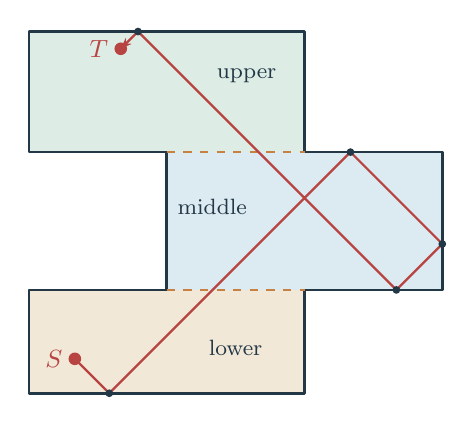
\begin{tikzpicture}[scale=1.75,line join=round]
\fill[piecezero] (0,-.75) rectangle (2,0);
\fill[pieceone] (1,0) rectangle (3,1);
\fill[piecetwo] (0,1) rectangle (2,1.875);
\draw[outline,line width=.9pt] (0,-.75)--(2,-.75)--(2,0)--(3,0)--(3,1)--(2,1)--(2,1.875)--(0,1.875)--(0,1)--(1,1)--(1,0)--(0,0)--cycle;
\draw[seam,dashed,line width=.8pt] (1,0)--(2,0) (1,1)--(2,1);
\draw[markcolor,line width=.8pt,-{Stealth[length=4pt]}] (1/3,-1/2)--(7/12,-3/4)--(7/3,1)--(3,1/3)--(8/3,0)--(19/24,15/8)--(2/3,7/4);
\foreach \p in {(7/12,-3/4),(7/3,1),(3,1/3),(8/3,0),(19/24,15/8)} \fill[outline] \p circle (.8pt);
\fill[markcolor] (1/3,-1/2) circle (1.3pt) node[left=1pt,font=\small] {$S$};
\fill[markcolor] (2/3,7/4) circle (1.3pt) node[left=1pt,font=\small] {$T$};
\node[font=\footnotesize,outline] at (1.5,-.42) {lower};
\node[font=\footnotesize,outline] at (1.33,.6) {middle};
\node[font=\footnotesize,outline] at (1.58,1.55) {upper};
\end{tikzpicture}
\caption{The room for $d=g=1$, $h_-=3/4$, and $h_+=7/8$, with portals dashed. The path joins $S=(1/3,-1/2)$ to $T=(2/3,7/4)$ with five reflections: the lower wall, three middle walls, and the upper wall. Section~\ref{sec:charts} explains this path as a three-pass chart with effective depths $1$ and $1$.}
\label{fig:room}
\end{figure}

\begin{remark}
The theorem covers only pairs with one point in each outer chamber. It gives no uniform bound on reflections. It doesn't address other interior pairs, other polygons, or the minimum wall count of a room with a dark pair.
\end{remark}

\paragraph{Related work.} The literature check for this draft found no exact statement of Theorem~\ref{thm:main} in the sources examined. Historical novelty remains to be confirmed. All angles of $P$ are rational multiples of $\pi$, so $P$ lies within the established theory of rational billiards. The finite-blocking and marked-point classifications of Monteil \cite{Monteil2005} and of Apisa and Wright \cite{ApisaWright2021} could imply the theorem through a further argument. This note doesn't exclude that route. Hubert, Schmoll, and Troubetzkoy study non-illuminated points on Veech surfaces \cite{HST2008}. The literature check reached only the abstracts of that paper and Monteil's paper. Davis poses illumination of a C-shaped pentomino as a course exercise \cite{Davis2016}, which is nearby prior art. The four-copy unfolding of $P$ has genus 5, so a theorem limited to genus 2 doesn't apply directly.

\section{Reduction to the left portions}\label{sec:reduction}
Scale $x$ by $1/d$ and $y$ by $1/g$. Every wall is axis-parallel, so each reflection still reverses one velocity component. Corner avoidance also persists. Assume $d=g=1$ for the rest of this note.

\begin{lemma}[L-shaped rooms]\label{lem:L}
Let $0<w<A$ and $0<c<C$, and let $R=([0,A]\times[0,c])\cup([0,w]\times[c,C])$. Let $p=(p_1,p_2)$ have $w<p_1<A$ and $0<p_2<c$, and let $p'=(p_1',p_2')$ have $0<p_1'<w$ and $c<p_2'<C$. Then $R$ has a corner-free trajectory from $p$ to $p'$ along which $y$ strictly increases.
\end{lemma}
\begin{proof}
Put $\rho=(p_2'-c)/(c-p_2)$ and $h=-\rho p_1$. The set $E=\{\pm p_1'+2mw:m\in\mathbb{Z}\}$ has alternating gaps $2p_1'$ and $2(w-p_1')$, both less than $2w$. Choose $x\in E$ with $0<|x-h|\le w$. If $x>h$, set $(X,X')=(p_1,x)$. Otherwise, set $(X,X')=(-p_1,-x)$. The segment from $(X,p_2)$ to $(X',p_2')$ crosses $y=c$ at $\kappa=|x-h|/(1+\rho)\in(0,w)$. Under $y=c$, its $x$-coordinate stays in $(-A,A)$, so a fold in $x=0$ gives at most one reflection. Over $y=c$, the triangular fold of period $2w$ fixes $\kappa$ and sends $X'$ to $p_1'$. Each contact lies in a wall interior.
\end{proof}

If $s,t>1$, or if one of them equals $1$ and the other exceeds $1$, the straight segment from $S$ to $T$ lies in $P$. If $s<1<t$, apply Lemma~\ref{lem:L} with $(\xi,\eta)=(y+h_-,2-x)$, $w=h_-$, $A=h_-+1+h_+$, $c=1$, and $C=2$, from $T$ to $S$. The resulting path reflects only at horizontal walls, and all of them are actual walls of $P$. If $t<1<s$, reflect in $y=1/2$ and reverse the path. Only the following case remains:
\begin{equation}\label{eq:domain}
0<s\le 1,\qquad 0<t\le 1.
\end{equation}

\section{Folding charts and cap transfer}\label{sec:charts}
Let $F$ be the triangular wave with $F(x)=x$ on $[0,2]$, $F(x)=4-x$ on $[2,4]$, and period 4. Fix \emph{effective depths} $U,V>0$ and a pass count $\ell\in\{1,3\}$. Choose $u\in\{0,2\}$, $\varepsilon=\pm1$, $M\in\mathbb{Z}$, and $c\in\{1,3\}$. Set
\begin{equation}\label{eq:line}
H=U+\ell+V,\qquad L=u+\varepsilon t+4M,\qquad X(z)=s+(L-s)\frac{z+U}{H},\qquad E_j=X(j).
\end{equation}
The chart is \emph{admissible} if $(E_0,E_\ell)$ modulo 4 lies in the open box of Table~\ref{tab:boxes}. If $\ell=3$, it must also satisfy the \emph{ledge guards}: $E_1$ and $E_2$ modulo 4 lie in $(c+1,c+2)\cup(c+2,c+3)$.

\begin{table}[ht]
\centering
\begin{tabular}{cccc}
\hline
$(u,c)$ & $E_0$ modulo 4 & $E_\ell$ modulo 4 & Portal value\\
\hline
$(0,1)$ & $(1,2)$ & $(1,2)$ & $X$ at both portals\\
$(0,3)$ & $(2,3)$ & $(2,3)$ & $4-X$ at both portals\\
$(2,1)$ & $(1,2)$ & $(0,1)$ & $X$, then $2-X$\\
$(2,3)$ & $(2,3)$ & $(3,4)$ & $4-X$, then $X-2$\\
\hline
\end{tabular}
\caption{Compatible portal boxes. Residues are taken in $[0,4)$.}
\label{tab:boxes}
\end{table}

An \emph{outer-simple} connection from $(s,-U)$ to $(t,1+V)$ lives in the room with unbounded outer strips, $([0,2]\times(-\infty,0])\cup([1,3]\times[0,1])\cup([0,2]\times[1,\infty))$. It is corner-free and crosses each portal strictly. Before its first crossing and after its last crossing, it reflects only at vertical walls. Between those crossings, it stays in the middle rectangle.

\begin{lemma}\label{lem:chart}
Each admissible chart gives an outer-simple connection from $(s,-U)$ to $(t,1+V)$.
\end{lemma}
\begin{proof}
Use horizontal position $F(X)$ for $z\le0$, $1+F(X-c)$ for $0\le z\le\ell$, and $F(X-u)$ for $z\ge\ell$. Use height $y=z$ for $z\le 0$ and $y=z-\ell+1$ for $z\ge\ell$. For $\ell=1$, use $y=z$ on the middle interval. For $\ell=3$, use $y=z$, $2-z$, and $z-2$ on $[0,1]$, $[1,2]$, and $[2,3]$. Table~\ref{tab:boxes} shows that adjacent horizontal formulas agree in value and derivative at each portal, with value in $(1,2)$. The endpoints are $F(s)=s$ and $F(L-u)=t$. For $\ell=3$, the ledge guards put the horizontal position at $z=1,2$ in $(2,3)$, so those contacts are smooth reflections at the middle ledges. The guards exclude $x=2$ and $x=3$ there. So every fold kink occurs away from the portal and ledge heights, and it is a smooth reflection at a vertical wall.
\end{proof}

Figure~\ref{fig:room} uses $\ell=3$, $U=V=1$, $u=2$, $\varepsilon=-1$, $M=1$, and $c=1$, after the transfer in Lemma~\ref{lem:cap}.

\begin{lemma}[Cap transfer]\label{lem:cap}
Let $A\in\{a,2h_--a\}$ and $B\in\{b,2h_+-b\}$. If an outer-simple connection joins $(s,-A)$ to $(t,1+B)$, then $S$ illuminates $T$ in $P$.
\end{lemma}
\begin{proof}
If $A=2h_--a$, replace the height $z$ by $-2h_--z$ for $z<-h_-$. This sends the start to $S$ and adds one contact with the lower wall. Side-wall contacts away from that height remain legal. If the contact with the lower wall is a corner, the developed horizontal coordinate there is an even integer. The fold is even about that integer, and the heights $-A$ and $-a$ are symmetric about $-h_-$. So the path revisits $S$ at $z=-a$, after the corner. Discard the prefix that ends at that visit.

At the upper wall, use the mirror-image fold. If its contact is a corner, the same symmetry shows that the path reaches $T$ before that corner, so truncate there. The two edits occur outside the portals and don't change the middle portion. Finally, truncate at the first arrival at $T$.
\end{proof}

Call $(a,b)$, $(A,b)$, $(a,B)$, and $(A,B)$, with $A=2h_--a>a$ and $B=2h_+-b>b$, the four \emph{sheets} of the pair. An admissible chart on any sheet gives a connection in $P$.

\section{Equal effective depths}\label{sec:equal}
\begin{proposition}\label{prop:equal}
Assume~\eqref{eq:domain}. If a sheet has $U=V$, then that sheet has an outer-simple connection, so $S$ illuminates $T$.
\end{proposition}
\begin{proof}
Reflection in $y=1/2$ with reversal preserves the hypotheses and exchanges $s$ and $t$, so assume $t\le s$. Put $D=s-t\in[0,1)$ and $\alpha=U/(2U+1)\in(0,1/2)$. For $\ell=1$, $E_0=(1-\alpha)s+\alpha(\varepsilon t+u+4M)$ and $E_1=\alpha s+(1-\alpha)(\varepsilon t+u+4M)$.

\emph{Window A.} Take $(u,\varepsilon)=(2,-1)$, so $E_0+E_1\equiv D+2$. If $E_0\in(1+D,2)$, then $E_1\in(D,1)$, and the chart $(2,1)$ is admissible.

\emph{Window B.} Take $(u,\varepsilon)=(0,-1)$, so $E_0+E_1\equiv D$. If $E_0\in(2,2+D)$, then $E_1\in(2,2+D)$, and the chart $(0,3)$ is admissible.

If $\alpha$ is irrational, $E_0$ is dense modulo 4, so window A succeeds. Let $\alpha=p/q$ in lowest terms. Then $E_0$ runs over a grid of spacing $4/q$. For $q\ge 9$, one window has length at least $1/2>4/q$.

If $q$ is even and $(s,t)\ne(1,1)$, take $(u,\varepsilon,M)=(0,1,q/2)$. Both portal values lie in $(2,3)$, so the chart $(0,3)$ is admissible. If $q\ge6$ is even and $s=t=1$, window A has length $1>4/q$. If $q=4$ and $s=t=1$, then $U=1/2$, and the following path works:
\[
(1,-\tfrac12)\to(\tfrac52,1)\to(3,\tfrac12)\to(\tfrac52,0)\to(1,\tfrac32).
\]
Both portal crossings occur at $x=3/2$.

If $q=3$, then $U=1$. Put $v=(6-s-t)/5$. The following three-reflection path is legal, where $(3,\eta)$ is the contact with the right wall:
\[
(s,-1)\to(s+v,0)\to(s+2v,1)\to(3,\eta)\to(t+2v,0)\to(t+v,1)\to(t,2).
\]
Indeed $1<s+v,\,t+v<2$ and $2<s+2v,\,t+2v<3$ on~\eqref{eq:domain}, and $s+2v+t+2v+v=6$.

For $q=5,7$, each entry of Table~\ref{tab:small} lists a chart and its four guards, each meaning a strictly positive value. These guards hold on $0<t\le s\le1$ under the stated condition. On a sheet, the $q=3$ and $q=4$ paths are outer-simple, as are all charts, so Lemma~\ref{lem:cap} applies.
\end{proof}

\begin{table}[ht]
\centering
\small
\begin{tabular}{cccccl}
\hline
$\alpha$ & Condition & $(u,\varepsilon)$ & $M$ & $c$ & Guards\\
\hline
$1/5$ & all & $(2,-1)$ & 1 & 1 & $4s-t+1,\ 4-4s+t,\ s-4t+4,\ 4t-s+1$\\
$2/5$ & all & $(2,-1)$ & 1 & 3 & $3s-2t+2,\ 3-3s+2t,\ 2s-3t+3,\ 3t-2s+2$\\
$2/7$ & all & $(2,-1)$ & 5 & 3 & $5s-2t+2,\ 5-5s+2t,\ 2s-5t+5,\ 5t-2s+2$\\
$3/7$ & all & $(2,-1)$ & 5 & 1 & $4s-3t+3,\ 4-4s+3t,\ 3s-4t+4,\ 4t-3s+3$\\
$1/7$ & $s<6t$ & $(2,-1)$ & 3 & 3 & $6s-t,\ 7-6s+t,\ s-6t+7,\ 6t-s$\\
$1/7$ & $s\ge6t$, $6s+t>2$ & $(0,1)$ & 3 & 3 & $6s+t-2,\ 9-6s-t,\ s+6t+2,\ 5-s-6t$\\
$1/7$ & $s\ge6t$, $6s+t\le2$ & $(2,1)$ & 2 & 1 & $6s+t+3,\ 4-6s-t,\ s+6t+4,\ 3-s-6t$\\
\hline
\end{tabular}
\caption{Explicit charts for equal depths with denominators 5 and 7.}
\label{tab:small}
\end{table}

\section{Irrational vertical data}\label{sec:irrational}
On a sheet $(U,V)$ with $\ell=1$, put $\alpha=U/H$ and $\beta=(U+1)/H$. The depths are rational exactly when both phases are rational.

\begin{proposition}\label{prop:irrational}
Assume~\eqref{eq:domain}. If one of $a,b,h_-,h_+$ is irrational, then $S$ illuminates $T$.
\end{proposition}
\begin{proof}
Take a sheet with an irrational depth. If $a$ or $b$ is irrational, use $(a,b)$. Otherwise, use $(A,b)$ or $(a,B)$. Reflection in $y=1/2$ with reversal maps charts to charts, so assume $t\le s$. If $(\alpha,\beta)$ satisfies no integer relation, Kronecker's theorem puts $M(\alpha,\beta)$ densely in the torus, and the box $(1,2)^2$ is reached.

Otherwise, the integer relations $m\alpha+n\beta=r$ form a cyclic group with primitive generator $(m,n,r)$, because one phase is irrational. By duality, the closure of the orbit is the full level set
\begin{equation}\label{eq:level}
mE_0+nE_1\equiv C\pmod 4,\qquad C=(m+n-r)s+r\varepsilon t+ru,
\end{equation}
including all its components. A box of Table~\ref{tab:boxes} has an open integer-endpoint image $(\mathrm{lo},\mathrm{hi})$ of length $|m|+|n|$ under $(x,y)\mapsto mx+ny$. It meets the closure exactly when $\mathrm{lo}<C+4k<\mathrm{hi}$ for some $k\in\mathbb{Z}$. Density then gives a finite $M$ with an admissible chart.

If $|m|+|n|\ge5$, this always holds for the box $(1,2)^2$. There are 30 primitive triples with $|m|+|n|\le4$. Certificate C1 covers $0<t\le s\le1$ for each triple. The only uncovered point is $s=t=1$ on the rows $\alpha=1/2$ and $\beta=1/2$, that is, $U=V+1$ and $V=U+1$.

Those equations can't hold on a sheet with exactly one irrational depth. So the remaining case uses the sheet $(a,b)$ with $s=t=1$ and, up to reflection and reversal, $b=a+1$. Then the following path is legal, where $h=h_+>b$:
\[
(1,-a)\to(2,h-a)\to(2-b/h,1+h)\to(1,1+b).\qedhere
\]
\end{proof}

\section{Rational vertical data and the proof of Theorem~\ref{thm:main}}\label{sec:rational}
The proof combines one support theorem, one rectangle classification, and one uniform sampling bound. These steps leave a finite list of rooms.

\begin{lemma}[Finite sampling]\label{lem:sampling}
Let $\alpha=A_0/q$ and $\beta=C_0/q$, with $\gcd(A_0,C_0,q)=1$.
\begin{enumerate}
\item If $q>100$ and no nonzero $(m,n)$ with $|m|+|n|\le4$ has $m\alpha+n\beta\in\mathbb{Z}$, then every translate of the orbit $\{4j(\alpha,\beta)\}$ modulo 4 meets every open unit square.
\item For a primitive relation $(m,n,r)$, the orbit visits every component of its level set, at spacing $4/q$ in the tangent parameter of $(-n,m)$.
\end{enumerate}
\end{lemma}
\begin{proof}
The lattice $\Lambda=\{(m,n):mA_0+nC_0\equiv0\pmod q\}$ has index $q$. An area argument with $\ell^1$ diamonds gives a shortest vector of $\ell^1$ length $w\le\sqrt{2q}$. Under the hypothesis of part~1, $w\ge5$. The relation generated by that vector is primitive. Its level set is a union of $g=\gcd(m,n)$ parallel circles. The orbit has order $q$ and moves among the circles by $r$ modulo $g$, with $\gcd(r,g)=1$. This proves part~2. Any open unit square contains a tangent segment of Euclidean length $(w-4)/w$. The orbit spacing is at most $4w/q$, so a hit follows when $q>4w^2/(w-4)$. That bound holds for $5\le w\le\sqrt{2q}$ and $q>100$.
\end{proof}

\begin{proposition}[Finite support]\label{prop:support}
Let $0<s,t\le1$ and $U,V>0$. If no one-pass chart is admissible on $(U,V)$, then $(U,V)$ lies on one of the ten lines
\[
\begin{gathered}U=1,\quad V=1,\quad V=U+1,\quad U=V+1,\quad V=2U+1,\\ U=2V+1,\quad V=2U+2,\quad U=2V+2,\quad V=3U+1,\quad U=3V+1,\end{gathered}
\]
or it is one of the eleven points $(\tfrac12,\tfrac12)$, $(\tfrac15,\tfrac35)$, $(\tfrac35,\tfrac15)$, $(3,5)$, $(5,3)$, $(\tfrac13,\tfrac73)$, $(\tfrac73,\tfrac13)$, $(\tfrac17,\tfrac37)$, $(\tfrac37,\tfrac17)$, $(5,8)$, $(8,5)$.
\end{proposition}
\begin{proof}
Suppose $(U,V)$ lies off the ten lines. If a depth is irrational, the proof of Proposition~\ref{prop:irrational} gives a chart, because its exceptions lie on the lines $V=U+1$ and $U=V+1$. So the phases are rational with denominator $q$. If there is no relation of $\ell^1$ norm at most 4, Lemma~\ref{lem:sampling} leaves $q\le100$. Otherwise, the phases satisfy one of the 30 short relations. Ten of these are the listed lines. The other 20 have a closed-square cover at phase margin $\eta=1/8$ (certificate C2). Tangent spacing then gives a chart when $q>16(|m|+|n|)$, so $q\le64$ remains. Certificate C3 exhausts the finite remainder of 119{,}740 phase pairs on the continuous endpoint square. Exactly eleven pairs keep a nonempty complement, and they are the eleven listed points.
\end{proof}

The support is a necessary condition only. A depth pair in the support needn't fail, and failure of a chart isn't darkness.

\begin{proof}[Proof of Theorem~\ref{thm:main}]
By Section~\ref{sec:reduction}, assume~\eqref{eq:domain}. By Proposition~\ref{prop:irrational}, assume $a,b,h_-,h_+$ are rational. Suppose $S$ doesn't illuminate $T$.

\emph{Step 1: rectangles.} No sheet has an admissible chart, so Proposition~\ref{prop:support} puts the four corners $(a,b)$, $(A,b)$, $(a,B)$, and $(A,B)$ of a rectangle in the support. By Proposition~\ref{prop:equal}, no sheet has equal depths.

\emph{Step 2: classification.} The eleven points have both coordinates different from $1$. So a coordinate slice through one of them meets each line in at most one point. A rectangle with such a corner therefore has finitely many possibilities. Suppose all corners lie on lines. Exact elimination over the $10^4$ line assignments (certificate C4) gives 90 one-parameter affine families, 288 isolated points, and no higher-dimensional solution. Sixteen families have an equal-depth sheet identically, which leaves 74 families.

\emph{Step 3: uniform margin.} On a family, each sheet has a fixed primitive relation in its phases. For $\ell=1$, this is the short relation of its line. For $\ell=3$, put $\alpha_3=U/H$ and $\delta=1/H$. Then $m\alpha_3+n\delta=r$ gives
\[
mE_0+nv\equiv(m-r)s+r\varepsilon t+ru\pmod 4,\qquad v=\frac{L-s}{H}.
\]
Shrink every portal and ledge interval by $\eta=1/8$. Certificate C5 shows that, for each of the 74 families, one-pass and three-pass windows together cover the closed square $[0,1]^2$ with 324 clauses. A shrunken window contains an open tangent segment of length at least $2\eta/K$, with $K=\max(|m|,|n|)$ for $\ell=1$ and $K=\max_{0\le j\le3}|jm-n|$ for $\ell=3$. By Lemma~\ref{lem:sampling}(2), a strict hit occurs when the phase denominator exceeds $2K/\eta$, and each such cutoff is at most $64$. For depths $U=p/D$ and $V=r'/D$ in lowest joint terms, the denominators are $q_1=p+r'+D$ and $q_3=q_1+2D>q_1$. So some sheet has $q_1\le64$, and that sheet fixes the family parameter.

\emph{Step 4: finite list.} Steps 1--3 leave a finite list of rooms. Certificate C6 enumerates it: 22{,}328 family members, 44 further isolated rectangles, and 166 further rectangles through the eleven points, 22{,}538 in all.

\emph{Step 5: finite cover.} For each listed room, a chart condition is a conjunction of 4 or 8 strict rational affine guards in $(s,t)$, using
\[
X(j)=\frac{(q-p-jD)s+\varepsilon(p+jD)t+(p+jD)(u+4M)}{q},\qquad q=p+r'+\ell D.
\]
Certificate C7 begins with $[0,1]^2$ and subtracts these open sets exactly, keeping boundary segments and isolated points. It discards a piece only when the piece lies in $\{s=0\}$ or $\{t=0\}$. Every final complement is empty, so every pair in~\eqref{eq:domain} has a chart. By Lemma~\ref{lem:chart} and Lemma~\ref{lem:cap}, $S$ illuminates $T$, which contradicts the supposition.
\end{proof}

\section{Certificates and verification status}\label{sec:status}
All certificates use exact rational arithmetic. They contain no floating-point tolerances and no endpoint grids. Table~\ref{tab:certs} lists them. A count in the table is a reproducibility record, not a proof step by itself.

\begin{table}[ht]
\centering
\small
\begin{tabular}{clp{7.1cm}}
\hline
ID & Used in & Claim and exact data\\
\hline
C1 & Prop.~\ref{prop:irrational} & 30 short relations cover $0<t\le s\le1$, except $s=t=1$ on two rows.\\
C2 & Prop.~\ref{prop:support} & 20 of 30 relations cover the closed square at $\eta=1/8$.\\
C3 & Prop.~\ref{prop:support} & 115{,}408 phase pairs with $q\le100$ and 4{,}332 pairs on good lines. Exceptions: 2 and 9.\\
C4 & Step 2 & $10^4$ assignments give 90 families and 288 isolated points.\\
C5 & Step 3 & 74 families and 324 clauses cover at $\eta=1/8$. Maximum cutoff: 64.\\
C6 & Step 4 & 22{,}538 rooms. Maximum periods: $q_1=750$ and $q_3=752$.\\
C7 & Step 5 & 770{,}912 saved clauses and 3{,}085{,}728 integer guard identities. Three-pass clauses occur in 490 rooms.\\
\hline
\end{tabular}
\caption{Computer certificates used in the proof.}
\label{tab:certs}
\end{table}

\paragraph{Review.} Two separate OpenAI Codex agent sessions wrote and reviewed the proof. The reviewing session read the hand arguments and wrote its own exact checkers for each certificate. It reproduced the finite list and replayed every C7 clause, then accepted the whole theorem on 6 November 2026. The authoring session checked 2{,}043 prescribed physical paths with exact arithmetic, and the reviewing session checked 153. These paths support the hand geometry, and they don't replace the quantified cover. A separate Claude session reviewed the L-room lemma. This review is AI review of a computer-assisted proof. It isn't formal verification, and no external expert has refereed it.

\paragraph{Data availability.} The proof records, exact checkers and certificate download instructions are in the project repository: \url{https://github.com/peytonprogrammer/illumination-problem}. See \texttt{docs/DATA.md} and \texttt{docs/REPRODUCIBILITY.md}. Access follows the repository policy; this draft does not claim a public supplement.

\paragraph{Open questions.} A hand proof of certificates C1--C7 would remove the computer dependence. It's also open whether covering or periodic-point theory gives a shorter proof. The theorem doesn't settle other interior pairs in $P$.

\section*{Acknowledgments}
The authors used OpenAI Codex agents to develop and review the proof, and Anthropic's Claude to prepare this manuscript. The authors remain responsible for its content.

\begin{thebibliography}{9}
\bibitem{ApisaWright2021}
P.~Apisa and A.~Wright, ``Marked points on translation surfaces,''
\emph{Geometry \& Topology} \textbf{25} (2021), 2913--2961.
\url{https://arxiv.org/abs/1708.03411}.

\bibitem{Davis2016}
D.~Davis, \emph{Math 424: Geometry, surfaces and billiards}, problem set, Williams College, Fall 2016, problem 6(b).
\url{https://math.williams.edu/files/2016/05/424-problems-all.pdf}.

\bibitem{HST2008}
P.~Hubert, M.~Schmoll, and S.~Troubetzkoy, ``Modular fibers and illumination problems,''
\emph{International Mathematics Research Notices} \textbf{2008}, rnn011.
\url{https://arxiv.org/abs/math/0602394}.

\bibitem{LMW2016}
S.~Lelièvre, T.~Monteil, and B.~Weiss, ``Everything is illuminated,''
\emph{Geometry \& Topology} \textbf{20} (2016), 1737--1762.
\url{https://arxiv.org/abs/1407.2975}.

\bibitem{Monteil2005}
T.~Monteil, ``On the finite blocking property,''
\emph{Annales de l'Institut Fourier} \textbf{55} (2005), 1195--1217.
\url{https://www.numdam.org/item/AIF_2005__55_4_1195_0/}.

\bibitem{Tokarsky1995}
G.~W. Tokarsky, ``Polygonal rooms not illuminable from every point,''
\emph{The American Mathematical Monthly} \textbf{102} (1995), no.~10, 867--879.
\url{https://doi.org/10.1080/00029890.1995.12004679}.

\bibitem{Wolecki2024}
A.~Wolecki, ``Illumination in rational billiards,''
\emph{arXiv:1905.09358v3} (2024).
\url{https://arxiv.org/abs/1905.09358v3}.
\end{thebibliography}
\end{document}
